\documentclass[german]{cgspaper} % change option to 'english' to include english logo in \copyrightspace

\usepackage[ngerman]{babel} % comment out to use english in auto-generated section titles
\usepackage[utf8]{inputenc}
\usepackage[ruled]{algorithm}
\usepackage{algpseudocode}
\usepackage{url}

\title{Titel der Seminararbeit}
\author{John Doe\\ Universität Potsdam, Digital Engineering Fakultät, Hasso-Plattner-Institut}

% Konfiguration des Veranstaltungs-Feldes
\subject{%
    \textbf{Seminar Advanced Information Visualization}\\
    Sommersemester 2017\\
    Themenstellung und Anleitung:
    XX und Prof.\ Dr.\ Jürgen Döllner}

\begin{document}

% Definition des Teasers
\teaser{
    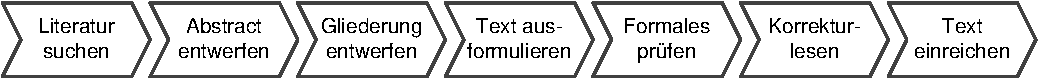
\includegraphics[width=0.9\textwidth]{graphics/prozess.pdf}
    \caption{Beispiel für einen Teaser: Schritte beim Erstellen eines fachwissenschaftlichen Beitrags. Ein Teaser dient als Blickfang schon auf der ersten Seite eines Artikels.}
    \label{fig:prozess}
}

\maketitle

%----------------------------------------------------------------
% Zusammenfassung
%----------------------------------------------------------------
\begin{abstract}
\end{abstract}

\copyrightspace % Erzeugt den Hinweis auf die Veranstaltung links unten

%----------------------------------------------------------------
% Einleitung
%----------------------------------------------------------------
\section{Einleitung}

%----------------------------------------------------------------
% Lehrstuhlkontext: 
% Diesen Abschnitt (in der deutschen bzw. englischen Fassung) übernehmen 
%----------------------------------------------------------------

\section{Kontext}
\label{sec:Kontext}
Die Betreuung im Rahmen der Seminartätigkeit erfolgte durch das Fachgebiet für Computergrafische Systeme, dessen Forschungsschwerpunkt die Prozessierung, Abbildung und interaktive Visualisierung massiver raumzeitlicher \cite{Oehlke2015,Buschmann2015,Buschmann2014,Maass2006} sowie abstrakter, hochdimensionaler Daten \cite{Limberger2017,Limberger2016,Wuerfel2015} ist. Dies beinhaltet neben neuartigen Algorithmen \cite{RichterKyprianidis2013,RichterBehrens2013,Glander2012}, Rendering-Techniken \cite{Semmo2016,Pasewaldt2014,Maass2006a,Doellner2005} und Interaktions-Metaphern \cite{Semmo2016a,Scheibel2016,Semmo2014} auch effiziente Datenstrukturen \cite{Scheibel2017,Richter2015} und Systemarchitekturen \cite{Klimke2014,Trapp2012,Klimke2010}, die anhand von real-weltlicher Datensätze und Anwendungsszenarien  \cite{Discher2016,Trapp2015,Engel2012} evaluiert werden. 

%\section{Context}
%\label{sec:Context}
%This course project was supervised by the Computer Graphics Systems Group whose main research interest includes the processing, mapping, and interactive visualization of massive spatio-temporal information \cite{Oehlke2015,Buschmann2015,Buschmann2014,Maass2006} and abstract high-dimensional information \cite{Limberger2017,Limberger2016,Wuerfel2015}. In particular, this comprises novel algorithms \cite{RichterKyprianidis2013,RichterBehrens2013,Glander2012}, rendering techniques \cite{Semmo2016,Pasewaldt2014,Maass2006a,Doellner2005}, and interaction metaphors \cite{Semmo2016a,Scheibel2016,Semmo2014}, as well as efficient data structures \cite{Scheibel2017,Richter2015} and system architectures \cite{Klimke2014,Trapp2012,Klimke2010} which are evaluated based on real-world data sets and application scenarios \cite{Discher2016,Trapp2015,Engel2012}.

%----------------------------------------------------------------
% Verwandte Arbeiten
%----------------------------------------------------------------
\section{Verwandte Arbeiten}
\label{sec:VerwandteArbeiten}
Praesent volutpat porttitor tristique. Curabitur finibus ut magna porttitor porttitor. Mauris non ipsum eu libero faucibus sodales. Vestibulum porta a purus vel pulvinar. Sed tellus sapien, imperdiet vitae dolor sed, imperdiet blandit purus. Pellentesque magna velit, condimentum at feugiat quis, mattis nec dui. Pellentesque et massa odio. Mauris sit amet commodo arcu. Suspendisse efficitur nulla nec ligula efficitur, et molestie orci suscipit. Quisque vehicula porta leo.

Donec sodales, justo ac fermentum lacinia, nisl nunc faucibus leo, quis rutrum tortor enim sit amet metus. Sed quis metus convallis, ultrices eros at, porta nisi. Aliquam erat volutpat. Phasellus faucibus dignissim diam, id porta lectus sagittis eget. In convallis rutrum turpis, sed viverra nisi laoreet cursus. Vestibulum ante ipsum primis in faucibus orci luctus et ultrices posuere cubilia Curae; Nunc id nisi ut sem ultricies dapibus. Sed ut quam non ex fermentum sodales. Nulla quam lorem, lacinia ac volutpat rhoncus, rhoncus a massa. Nunc posuere dapibus metus, vel maximus velit. Pellentesque sed lectus tristique, ornare lorem ut, hendrerit velit. Etiam fermentum ultricies nunc non volutpat. Vivamus fringilla vitae lacus non laoreet. Duis sit amet augue non mi luctus dignissim. In in tempor elit, vitae venenatis lectus. Aliquam erat volutpat.

%----------------------------------------------------------------
% Quellenverzeichnis
%----------------------------------------------------------------
\bibliographystyle{acmsiggraph}
\bibliography{foo-paper}

\end{document}
